\documentclass[a4paper,10pt]{article}

\usepackage{ifpdf}
\ifpdf
  \usepackage[pdftex]{graphicx}
  \graphicspath{{images/}}
\else
  \RequirePackage[dvipdfm, CJKbookmarks, bookmarks=true, bookmarksnumbered=true%
                unicode,%
             colorlinks,%
         citecolor=blue,%
             hyperindex,%
       plainpages=false,%
      pdfstartview=FitH]{hyperref}
  \AtBeginDvi{\special{pdf:tounicode UTF8-UCS2}}
  \usepackage[dvipdfm]{graphicx}
  \graphicspath{{images/}}
  \DeclareGraphicsExtensions{.eps}
\fi

%\RequirePackage{CJKutf8,CJKnumb,CJKulem}
\RequirePackage{CJKutf8,CJKnumb}
\RequirePackage{color,verbatim,cite}
\RequirePackage{texnames,makeidx,indentfirst}
\RequirePackage{amsmath,amssymb,amsfonts,bm,manfnt}
\RequirePackage{fancyhdr,titlesec,datetime}
\RequirePackage{wasysym,longtable,multirow,bigstrut}
\usepackage[section]{placeins}
\usepackage[left=2cm,right=2cm,top=2.5cm,bottom=2.6cm]{geometry}
\usepackage[caption=false,font=footnotesize]{subfig}

\AtBeginDocument{\begin{CJK*}{UTF8}{song}\CJKtilde\CJKindent\CJKcaption{utf8}}
\AtEndDocument{\end{CJK*}}

\setlength{\parskip}{0.75ex plus .2ex minus .5ex}
\renewcommand{\baselinestretch}{1.2}

\hypersetup {
    pdftitle={无线传感器网络中的密钥管理技术},
    pdfauthor={杨文博}
}

\title{无线传感器网络中的密钥管理技术}
\author{杨文博}

\begin{document}

\maketitle

\section{国内外研究现状调研}

虽然对密钥管理协议的研究已经有了多年的发展,对~WSN~密钥管理技术的系统研究大致开始于~2002~年。按照密钥分配方式的不同,我们可以将目前的几种流行方法~\cite{Lee2007}~大致分为三类:密钥子集交集、算术方法和分层的密钥管理协议,如图~\ref{wsn_keyman_1}~所示。

\begin{figure}[htbp]
  \centering
  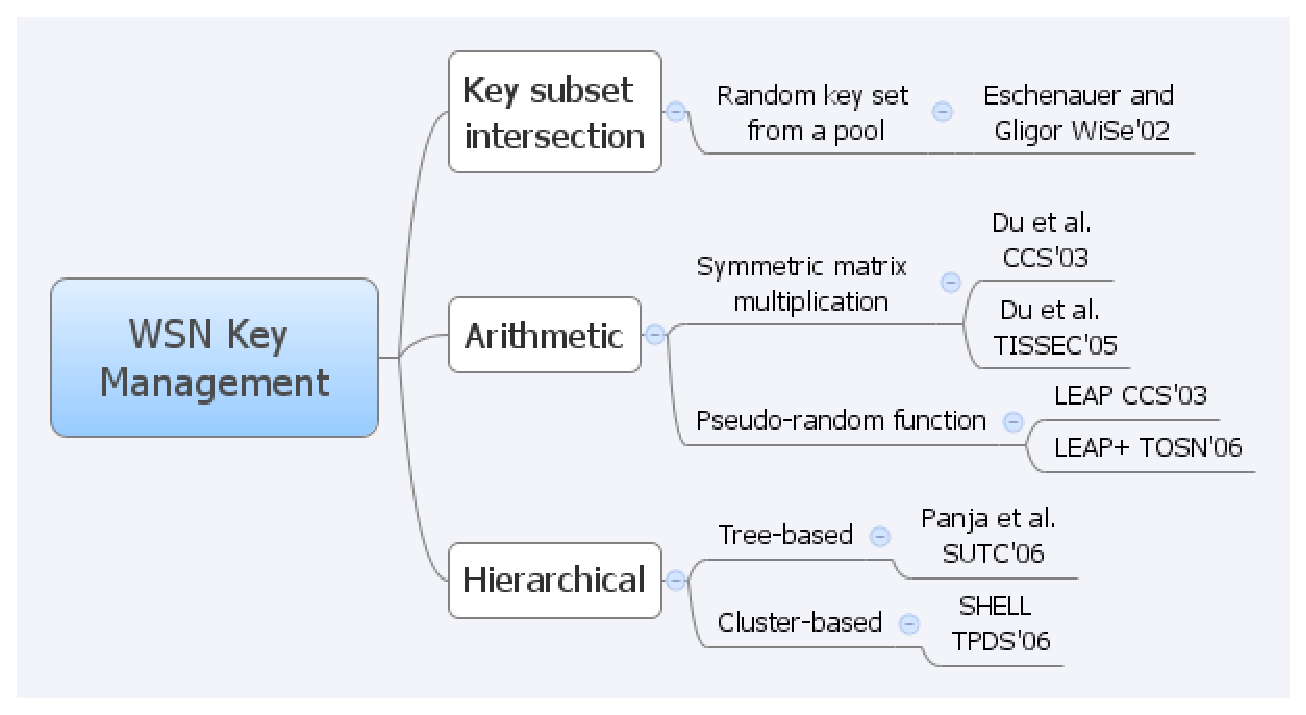
\includegraphics[width=.9\textwidth,keepaspectratio]{wsn_keyman_1}
  \caption{\label{wsn_keyman_1}~WSN~密钥管理协议}
\end{figure}

\begin{enumerate}

\item 密钥子集交集。为了减少对密钥存储的开销,节点可以仅仅存储部分而不是全网的对密钥信息,当需要通信时,利用子集交集得到通信密钥。L. Eschenauer~和~V. Gligor~提出了一个随机密钥子集的方案~\cite{Eschenauer2002}~。首先生成一个密钥池(密钥集),从中随机选择密钥子集存储到每个节点中。当有通信需要时,两个节点查看双方的密钥子集是否有交集,如果有就使用交集中的某密钥通信,否则通过中间节点中转通信。

\item 算术方法。W. Du~等提出一个基于对称矩阵的密钥子集方案~\cite{Du2003, Du2005}~。它采用了一个~Blom~的密钥预分配算法,基本思想是事先计算一个~(r+1)*N~阶的公开矩阵~G~,一个~(r+1)*(r+1)~阶的对称秘密矩阵~D,$A=(D*G)^T$~,则有~$A*G=(A*G)^T$,那么一方只需存储~A~的第~K~行,G~的第~K~列。双方就可以通过交换~G~的列,然后计算得双方的密钥。Du~的方案为了节省密钥存储开销,采用了多个秘密和公开矩阵的做法,每个节点存储这些秘密和公开矩阵的一个子集,如果它们有公共的公开矩阵,就可以直接生成密钥进行通信,否则需要间接通信;S. Zhu~等提出了一个混合的算法~LEAP(Localized Encryption and Authentication Protocol)\cite{Zhu2003}~,这个密钥管理算法提供了四种密钥的管理和分发:个体密钥(Individual Key)、组密钥(Group Key,其实文中意思是网络密钥)、簇密钥(Cluster Key)和对密钥(Pairwise Key)。个体密钥是预加载到节点中的,为了减少基站的存储开销,个体密钥可以用以节点~ID~和基站密钥~$K^m_s$~为参数的伪随机函数产生:$K^m_u=f_{K^m_s}(u)$;所有节点还将预置一个相同的初始化密钥$K_I$,每个节点以初始化密钥为参数生成一个主密钥$K_u=f_{K_I}(u)$,然后广播~ID~,当相邻两个节点:u, v,收到对方的~ID~时,就能计算出对密钥~$K_{uv}=f_{K_v}(u)=f_{f_{K_I}(v)}(u)=f_{K_u}(v)$;得到对密钥之后,簇头通过单播向所有节点传输簇密钥;全网的组密钥可以通过多跳或者多簇的方式传播给各个节点。在密钥更新算法方面,LEAP~使用~μTESLA~协议撤销某节点密钥,使用单向密钥链定期更新全网组密钥。S. Zhu~等在~\cite{Zhu2006}~中对~LEAP~进行改进,提出了~LEAP+~算法,将组密钥改成全局密钥(Global Key),在对密钥的建立方面,移除了对初始化密钥~$K_I$~的依赖,简单来说就是让~$K_I$~随时间变化,其它过程大致与~LEAP~一样。

\item 分层方法。B. Panja~等提出了一个基于树结构的组密钥分配协议~TGDH(Tree-based Group Deffie-Hellman)~\cite{Panja2006}~,其密钥分配的基本过程是整个网络形成一棵树,叶子节点生成随机数作为部分密钥(partical key),父节点根据子节点的部分密钥计算自己密钥,以此类推。分配密钥的过程由全局预加载的密钥加密,计算方法采用多方~DH~算法(Multi-party Deffie-Hellman)。更新组密钥的时候,由父节点向子节点发出一个插入或者移除某部分密钥的指令即可;M. Younis~等提出了一个基于分簇的算法~SHELL(Scalable, Hierarchical, Efficient, Location-aware, and Light-weight)\cite{Younis2006}。该算法比较复杂,其主要思想是簇头节点不是唯一的密钥管理节点,每个簇的密钥会由其它另外的簇头和自己的簇头共同管理。对每个簇中的节点使用~EBS(Exclusion Basis Systems)~算法来计算组密钥。

\end{enumerate}

\section{研究发展方向}

1. 多层次的密钥管理。目前来讲,单单是对密钥或者组密钥管理都不能满足一些需要,发展多层次的密钥管理有助于解决组播、数据融合等需求。

2. 健壮的密钥管理算法。目前健壮的密钥管理算法往往只提供了有限的密钥管理服务,提供了多层次密钥管理的协议都比较复杂,或者带来更大的开销。

\bibliographystyle{IEEEtran}
\bibliography{IEEEfull,wsn}

\end{document}

